\documentclass[12pt,dvipdfmx]{jarticle}
%\documentstyle[12pt,fleqn,epsf,iepaper,cite]{jarticle}
%\documentstyle[12pt,iepaper,eclepsf,oddchar]{jarticle}

\usepackage{colortbl}
\usepackage{multicol}
\usepackage{amsmath}
\usepackage{amssymb}
\usepackage{amsfonts}
\usepackage{mathbbol}
\newcommand{\bm}[1]{{\mbox{\boldmath $#1$}}}
\usepackage{cite}


\usepackage[dvipdfm]{graphicx}
\usepackage{iepaper}
\usepackage{epsf}
\usepackage{ccaption}
\usepackage{pdfpages}

\title{遺伝的アルゴリズムによる機械学習における\\疑似ラベル生成手法の提案}
\author{細川 岳大}
\gakuseki{}[B]  %卒論はB,修論はM
\group{知能情報第 1 グループ}            % 卒論の場合
\shidou{森 直樹 教授}                          % 卒論の場合
%\syusa{教授}                            % 修論の場合
%\hukusa{教授}{教授}

%図番号を「(section番号).(図番号)」とするため
\makeatletter
\renewcommand{\thefigure}{%
	\thesection.\arabic{figure}}
\@addtoreset{figure}{section}
\makeatother

\makeatletter
\renewcommand{\thetable}{%
	\thesection.\arabic{table}}
\@addtoreset{table}{section}
\makeatother

\makeatletter
\renewcommand{\theequation}{%
	\thesection.\arabic{equation}}
\@addtoreset{equation}{section}
\makeatother


\begin{document}
	\maketitle
	
	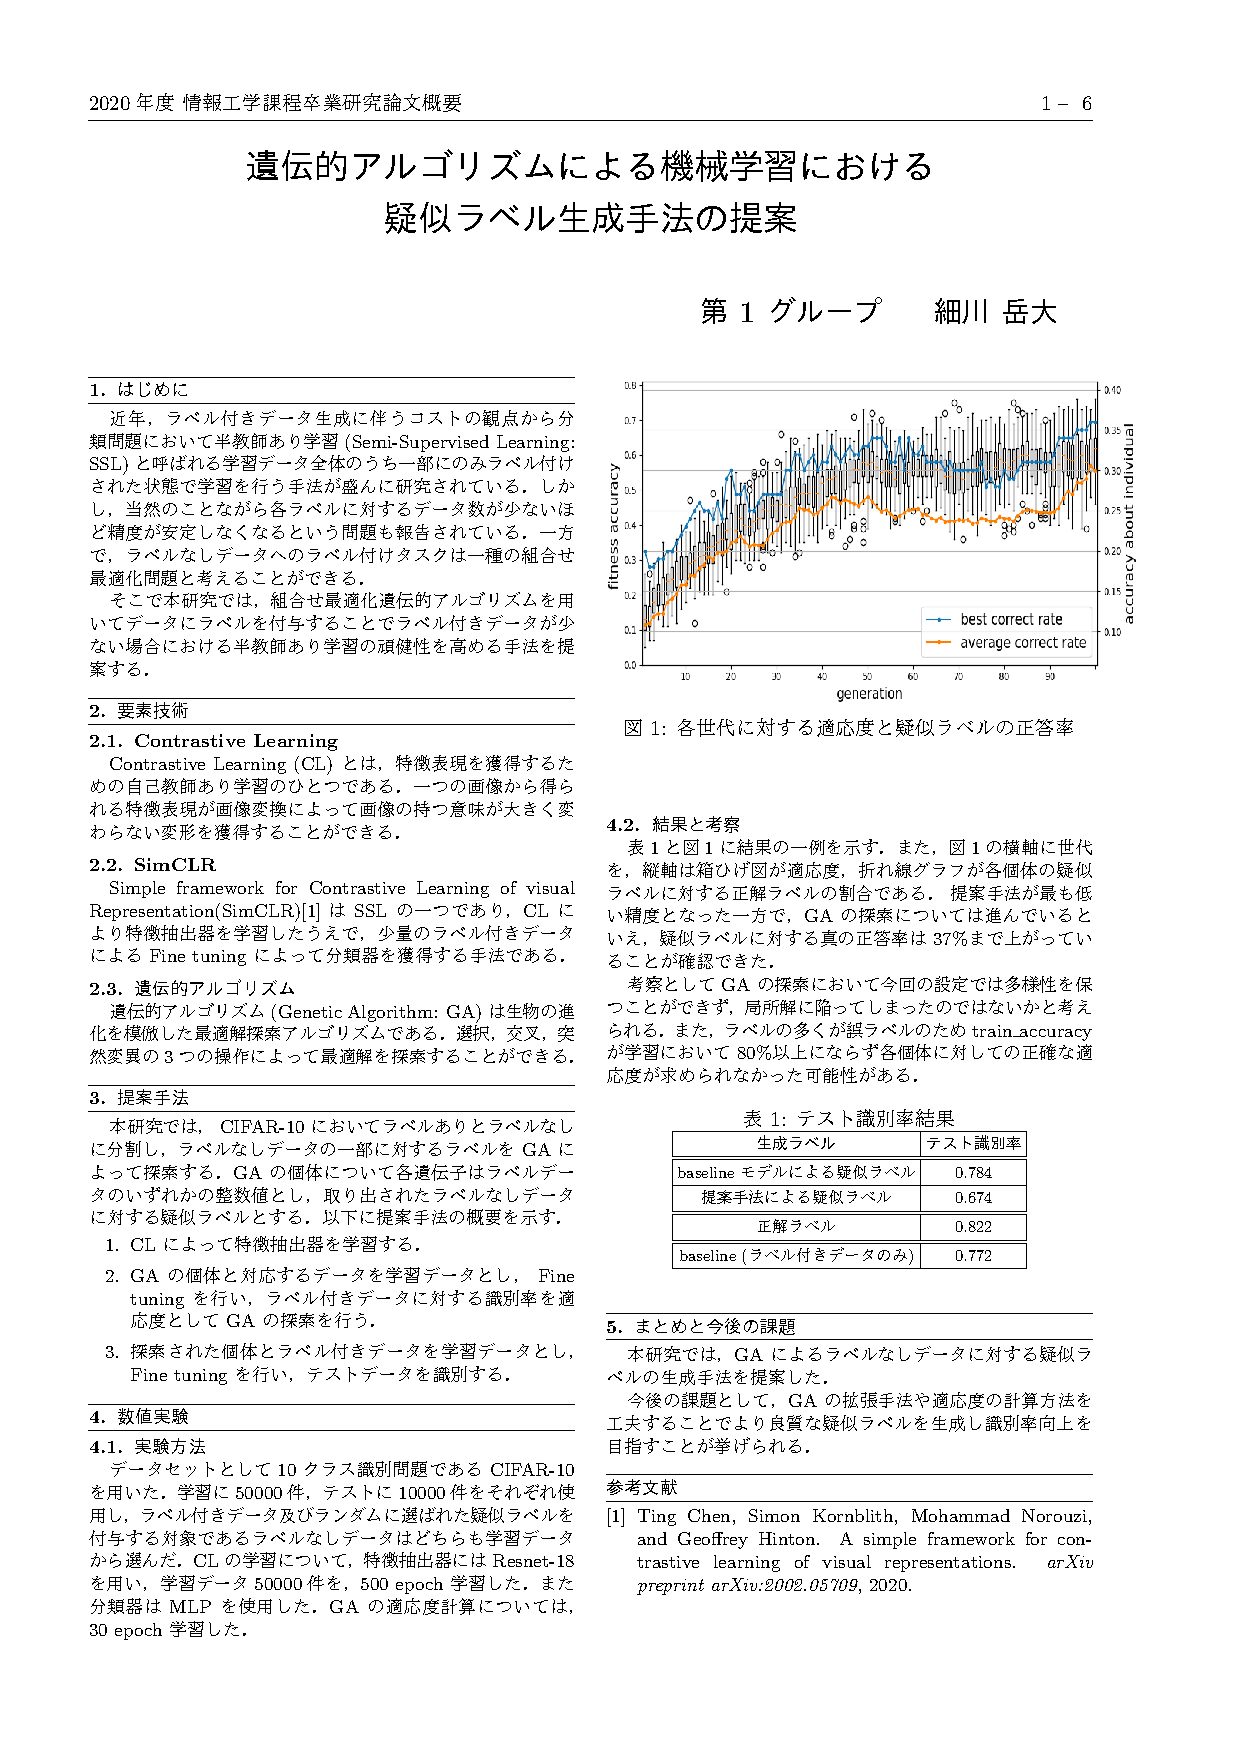
\includepdf[fitpaper]
	{../abstract/abstract_2020_final_hosokawa.pdf}
	\pagenumbering{roman}
	%%% 目次
	\tableofcontents
	\newpage
	%
	%% 図一覧
	\listoffigures
	\newpage
	
	%% 表一覧
	\listoftables
	\newpage
	
	\pagenumbering{arabic}
	
	% 文書開始
	\newpage
\changeindent{0cm}
\section{はじめに}
\changeindent{2cm}
近年,機械学習の発展に伴い,様々な分野への応用がされており
様々な新規データセットにおいて目覚ましい結果が報告されている.
また新規データセットを生成する際,分類問題では各データにふさわしいラベル付けをする必要があり,
ラベル付けには人の手が必要でありコストがかかる問題がある.
そこで半教師あり学習 (Semi-Supervised Learning: SSL)\cite{zhu2005semi}と呼ばれる
学習データ全体のうち一部にのみラベルが付与された状態で学習を行う手法が提案されており,
盛んに研究されており,全データにラベルが付与されている教師あり学習にも劣らない成果の報告\cite{sohn2020fixmatch}もある.しかし,当然のことながら各ラベルに対するデータ数が少ないほど精度が安定しなくなるという報告もされている.

一方,ラベルなしデータへのラベル付けタスクは一種の組合せ最適化問題と考えることができる.

本研究では,組合せ最適化遺伝的アルゴリズムを用いてデータにラベルを付与することでラベル付きデータが少ない場合における半教師あり学習の頑健
性を高める手法を提案する.

以下に本欄分の構成を示す.まず,2章では本研究で用いる要素技術につ
いて概説する.続いて3章で実験手法の提案をし,4章において実験結果と考察を
示す.5章で本研究の成果をまとめたうえで,今後の課題について述べる.


	\clearpage
	%要素技術
	\newpage
\changeindent{0cm}
\section{要素技術}
\changeindent{2cm}

本章では,実験に関連する要素技術について説明する.

\changeindent{0cm}
\subsection{半教師あり学習}
\changeindent{2cm}
半教師あり学習 (Semi Supervised Learning: SSL)\cite{zhu2005semi} は
大量のラベルなしデータと少量のラベル付きデータを用いて学習を行う手法である.

\changeindent{0cm}
\subsection{疑似ラベル}
\changeindent{2cm}
疑似ラベル (Pseudo Label)\cite{lee2013pseudo} はあるモデルによって予測されるラベルなしデータに対する暫定的なラベルである.
 SSL では疑似ラベルを付与したデータをラベル付きデータに混ぜて学習することで各ラベル同士に対する確率分布を粗密なものとして作用することで正則化の役割をする.
 

\changeindent{0cm}
\subsection{SimCLR}
\changeindent{2cm}
Simple framework for Contrastive Learning of visual Representation(SimCLR)\cite{chen2020simple} は SSL の一つである.
図\ref{fig:SimCLR}に概略図を示す.モデルの構造は Encoder,Projection Head,Classsifer
から構成されており, Encoder と Projection Head に対して,全データを用いて Contrastive Learning によって学習する.次に学習済みの Encoder と Classifer に対して,ラベル付きデータを用いて Classfier の学習を行う.最後にモデルの蒸留を行うことで最終的なモデルを得る.
\begin{figure}[h]
	\begin{center}
		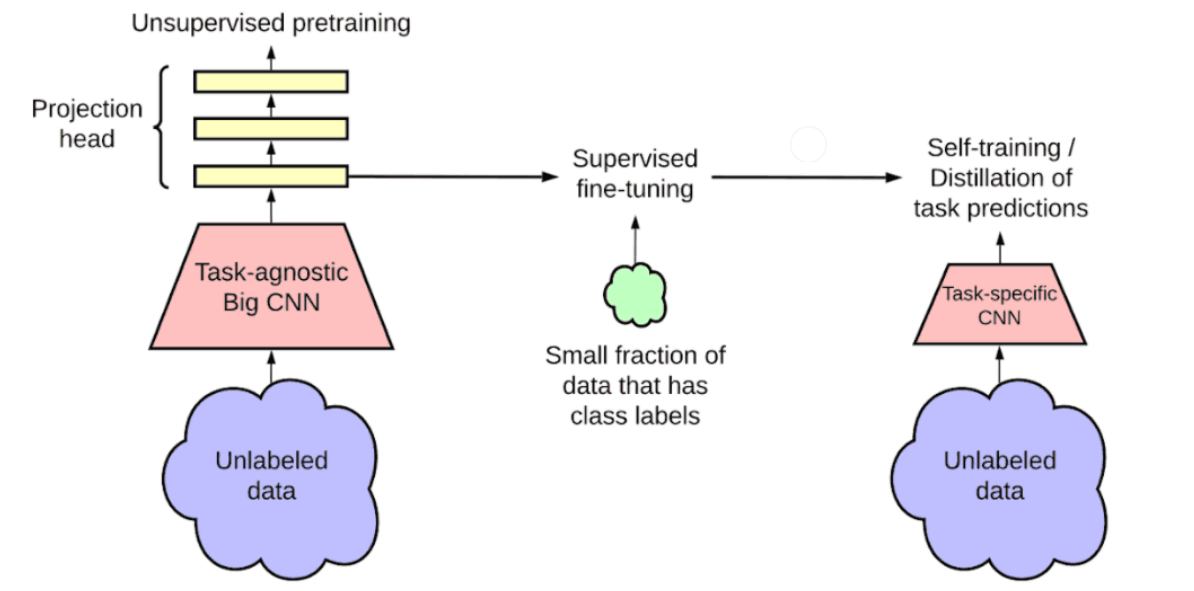
\includegraphics[scale=1.0]{./images/SimCLR.png}
		\caption{SimCLR の概略: 文献\cite{chen2020big}の Figure 3 を参照\label{fig:SimCLR}}
	\end{center}
\end{figure}

\changeindent{0cm}
\subsubsection{Cotrastive Learning}
\changeindent{2cm}
Contrastive Learning (CL)\cite{tian2020makes} とは特徴表現を獲得するための
自己教師あり学習のひとつである.
ある画像変換をした画像のペアについて元画像が一致するか否かを識別するタスクであり,
一つの画像から得られる特徴表現が画像変換によって
画像の持つ意味が大きく変化させない変形を獲得することができる.
具体的な方法について,バッチ内の画像枚数を $N$ 枚とすると, Data Augmentation によって2倍に増やしたとき,
各画像に対して正例は1枚,負例は $2(N-1)$ 枚となる.このとき特徴ベクトル間の距離として cos 類似度を用いて
式となる.また,正例との距離を小さくかつ,負例との距離を大きくするために正例のペア $(z_i,z_j)$ に対するロス $l_{i,j}$ は式で表され,
バッチ全体のロス $L$ 


\changeindent{0cm}
\subsection{ResNet}
\changeindent{2cm}
Residual Network (: ResNet)\cite{he2016deep} は Deep Neural Network (: DNN) のモデルの一つであり,
 DNNにおいて層を深くすることで発生する劣化問題及び勾配消失問題を解消するために残差についての学習を行うことを目的としている.図\ref{fig:ResBlock}に ResNet の構成要素である Residual Block の構造を示す.
2層の畳み込み層とショートカットの足し合わせた構造となっている.

\begin{figure}[h]
	\begin{center}
		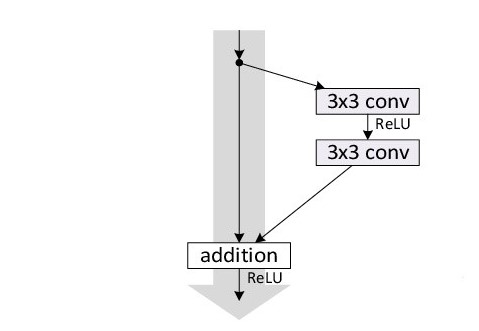
\includegraphics[scale=0.5]{./images/ResBlock.jpg}
		\caption{Residual Block の構造: 文献\cite{he2016identity}の Figure 2.(a) を参照\label{fig:ResBlock}}
	\end{center}
\end{figure}

\changeindent{0cm}
\subsection{Genetic Algorithm}
\changeindent{2cm}
\cite{whitley1994genetic}


\cite{murata1996multi}



CIFAR10\cite{krizhevsky2009learning}
	\clearpage
	
	
\newpage
\changeindent{0cm}
\section{提案手法}
\changeindent{2cm}
本研究では,ラベルなしデータに対する疑似ラベルを GA を用いて
探索する手法を提案する.
また以降,半教師あり学習のデータについて学習データである
ラベル付きデータとラベルなしデータをそれぞれ $D_{\rm l}$\ ,$D_{\rm ul}$\ ,
テストデータを $D_{\rm t}$ と呼ぶ.


\changeindent{0cm}
\subsection{個体設定}
\changeindent{2cm}
まず,$D_{\rm ul}$からランダムにいくつかデータを取り出し探索データとする.
ここで,GAの扱う個体は探索データに対する疑似ラベル群である.
探索データと各遺伝子座は一対一対応しており,
遺伝子型は対応するラベルを表す整数値である.
従って,遺伝子長は探索データ数となる.
以降探索データについて $D_{\rm s}$ と呼ぶ.

\changeindent{0cm}
\section{提案手法}
\changeindent{2cm}
以下に提案手法の手順を示す.

\begin{enumerate}
	\item モデルの事前学習
	\item 事前学習したモデルに入力データを $D_{\rm s}$ ,ラベルデータを各個体とし
	学習し,$D_{\rm l}$ の識別率を適応度として GA の探索を行う.
	\item $D_{\rm l}$ と探索された個体をラベルとして持つ $D_{s}$ とを合わせてラベル付きデータとして
	 SSL によって再学習を行い $D_{\rm t}$ を識別する.
\end{enumerate}

既存の疑似ラベルを用いた手法では $D_{\rm s}$ で学習されるモデルの精度に大きく影響されるが,提案手法では疑似ラベルはモデルの出力ではないため正答率があがり,結果として半教師あり学習による精度も改善されることが期待できる.


	\clearpage
	
	\newpage
\changeindent{0cm}
\section{数値実験}
\changeindent{2cm}

	\clearpage
	
	\newpage
\changeindent{0cm}
\section{まとめと今後の課題}
\changeindent{2cm}
本研究では,遺伝的アルゴリズムを用いてラベルなしデータに対する疑似ラベル生成手法の提案をした.
また,数値実験から探索された疑似ラベルを用いた学習において精度の低下を確認し,
遺伝的アルゴリズムによるラベル探索は非常に困難であることが分かった.

今後の課題として,遺伝的アルゴリズムのパラメータチューニング及び,
膨大な探索空間に有効に拡張されたアルゴリズムを使用するといった遺伝的アルゴリズムの改善と,
validation data も画像の水増しを行うことや一個体の学習に対するパラメータチューニングといった
適応度計算の改善の2点が挙げられる.




	\clearpage
	
	\newpage
\changeindent{0cm}
\acknowledgements
\changeindent{2cm}

本研究を進めるにあたりご指導,ご鞭撻を賜りました森直樹教授,岡田真助教授に深く感謝申し上げます.
また,発表スライドや本論文の作成にあたり添削及びアドバイスを下さったソフトウェア研究システムグループの皆様にも厚く御礼を申し上げ,
感謝の意を表します.
\begin{flushright}
	2021年2月26日
\end{flushright}

	
	% 参考文献
	\clearpage
	%\newpage
\changeindent{0cm}
\begin{thebibliography}{99}
 \changeindent{2cm}
\end{thebibliography}


	%\changeindent{0cm}
	\bibliographystyle{unsrt}
	\bibliography{reference}
	
	
	
\end{document}